\appendix
\appendixpage
\renewcommand{\thesection}{A.\arabic{section}}
\addappheadtotoc

\section{Extended Euclidean Algorithm}
\label{appendix:euclidean}

In the following pseudocode, $\text{leading\_zeros}(x)$ returns the number of leading zero bits in $x$.
Modern CPUs have a dedicated instruction for counting leading zeros.

Because the irreducible polynomial is of degree 64, the first Euclidean division iteration, in the first iteration of the Euclidean algorithm, is a special case.
As a 65-bit polynomial cannot fit in the 64-bit variable $b$, the first iteration is done manually, outside the loop.

\begin{algorithm}
\caption{Extended Euclidean Algorithm}
\begin{algorithmic}
\Function{ExtendedEuclidean}{$a$}

\State $\textbf{assert}\ a \neq 0$

\State \algorithmicif\ $a = 1$ \algorithmicthen\ \Return $1$ \algorithmicend \algorithmicif

\State $t \gets 0$
\State $\text{new\_t} \gets 1$
\State $r \gets \text{POLYNOMIAL}$ \Comment the irreducible polynomial, 65-th bit excluded
    \State $\text{new\_r} \gets a$

\State $r \gets r \oplus (\text{new\_r} \ll (\text{leading\_zeros}(\text{new\_r}) + 1))$
\State $\text{quotient} \gets 1 \ll (\text{leading\_zeros}(\text{new\_r}) + 1)$

\While{$\text{new\_r} \neq 0$}
    \While{$\text{leading\_zeros}(\text{new\_r}) >= \text{leading\_zeros}(r)$}
        \State $\text{degree\_diff} \gets \text{leading\_zeros}(\text{new\_r}) - \text{leading\_zeros}(r)$
        \State $\text{r} \gets r \oplus (\text{new\_r} \ll \text{degree\_diff})$
        \State $\text{quotient} \gets \text{quotient} | (1 \ll \text{degree\_diff})$
    \EndWhile
    \State $(r, \text{new\_r}) \gets (\text{new\_r}, r)$
    \State $(t, \text{new\_t}) \gets (\text{new\_t}, t \oplus \text{gf64\_multiply}(\text{quotient}, \text{new\_t}))$
    \State $\text{quotient} \gets 0$
\EndWhile
\State $\textbf{assert}\ r = 1$
\State \Return $t$
\EndFunction
\end{algorithmic}
\end{algorithm}

\section{Polynomial Transforms}
\label{appendix:transforms}

The inverse and forward transforms are almost identical, except the outer loop direction and the inner operations are reversed.

\begin{algorithm}[!hb]
    \caption{Transform Algorithms}
    \begin{algorithmic}
        \Function{InverseTransform}{\text{data}, \text{factors}}
            \For{$\text{step} \gets 0\ \textbf{to}\ \log_2(\text{len(data)}) - 1$}
                \State $\text{group\_len} \gets 2^{\text{step}}$
                \State $\text{group\_factors\_start} \gets \text{len(factors)} + 1 - \frac{\text{len(factors)} + 1}{2^{\text{step}}}$
                \For{$\text{group} \gets 0\ \textbf{to}\ \frac{\text{len(data)}}{2^{\text{step} + 1}} - 1$}
                    \For{$\text{x} \gets 0\ \textbf{to}\ \text{group\_len} - 1$}
                        \State $a \gets \text{group} \cdot \text{group\_len} \cdot 2 + x$
                        \State $b \gets a + \text{group\_len}$
                        \State $\text{data}[b] \gets \text{data}[b] + \text{data}[a]$
                        \State $\text{data}[a] \gets \text{data}[a] + \text{data}[b] \cdot \text{factors}[\text{group\_factors\_start} + \text{group}]$
                    \EndFor
                \EndFor
            \EndFor
        \EndFunction
    \end{algorithmic}

    \begin{algorithmic}
        \Function{ForwardTransform}{\text{data}, \text{factors}}
            \For{$\text{step} \gets \log_2(\text{len(data)}) - 1\ \textbf{down to}\ 0$}
                \State $\text{group\_len} \gets 2^\text{step}$
                \State $\text{group\_factors\_start} \gets \text{len(factors)} + 1 - \frac{\text{len(factors)} + 1}{2^{\text{step}}}$
                \For{$\text{group} \gets 0\ \textbf{to}\ \frac{\text{len(data)}}{2^{\text{step} + 1}} - 1$}
                    \For{$\text{x} \gets 0\ \textbf{to}\ \text{group\_len} - 1$}
                        \State $a \gets \text{group} \cdot \text{group\_len} \cdot 2 + x$
                        \State $b \gets a + \text{group\_len}$
                        \State $\text{data}[a] \gets \text{data}[a] + \text{data}[b] \cdot \text{factors}[\text{group\_factors\_start} + \text{group}]$
                        \State $\text{data}[b] \gets \text{data}[b] + \text{data}[a]$
                    \EndFor
                \EndFor
            \EndFor
        \EndFunction
    \end{algorithmic}

    \begin{algorithmic}
        \Function{PrecomputeFactors}{\text{pow}, \text{offset}}
            \State $\text{factors} \gets \text{new array of \GF{64} values of size } 2^{\text{pow}} - 1$
            \State $\text{factor\_idx} \gets 0$
            \For{$\text{step} \gets 0\ \textbf{to}\ \text{pow} - 1$}
                \State $\text{groups} \gets 2^{\text{pow} - \text{step} - 1}$
                \For{$\text{group} \gets 0 \text{ to } \text{groups} - 1$}
                    \State $\text{factors}[\text{factor\_idx}] \gets \hat{W}_{\text{step}}(\omega_{\text{group} \cdot 2^{\text{step} + 1}} + \omega_{\text{offset}})$
                    \State $\text{factor\_idx} \gets \text{factor\_idx} + 1$
                \EndFor
            \EndFor
            \State \Return $\text{factors}$
        \EndFunction
    \end{algorithmic}
\end{algorithm}

Notice that the transforms can use factors of a greater power than needed. To compute multiple transforms of different sizes with the same offset, only the factors for the largest size must be computed, and can be used for all smaller sizes.
This is very convenient for the error locator polynomial computation algorithm, which uses transforms of many different sizes.

The precomputed factors require $O(n \log n)$ time and space complexity.

\section{Formal Derivative}
\label{appendix:derivative}

The formal derivative also has time complexity $O(n \log n)$, but unlike the transforms, the factors only require $O(\log n)$ space.

\begin{algorithm}
    \caption{Formal Derivative Algorithm}
    \begin{algorithmic}
        \Function{PrecomputeDerivativeFactors}{\text{pow}}
            \State $\text{assert}\ 0 \leq \text{pow} \le 64$
            \State $\text{factors} \gets \text{new array of \GF{64} values of size } \text{pow}$
            \For{$l \gets 1\ \textbf{to}\ \text{pow} - 1$}
                \For{$j \gets 2^{l - 1}\ \textbf{to}\ 2^l - 1$}
                    \State $\text{factors}[l] \gets \text{factors}[l] * \omega_j$
                \EndFor
                \If{$l + 1 \neq \text{pow}$}
                    \State $\text{factors}[l + 1] \gets \text{factors}[l]$
                \EndIf
                \State $\text{factors}[l] \gets \text{factors}[l] / W_l(2^l)$
            \EndFor
            \State \Return $\text{factors}$
        \EndFunction
    \end{algorithmic}
    \begin{algorithmic}
        \Function{FormalDerivative}{\text{data}, \text{factors}}
            \For{$i \gets 0\ \textbf{to}\ \text{len(data) - 1}$}
                \For{$\text{bit} \gets 0\ \textbf{to}\ \log_2(\text{len(data)})$}
                    \If{$i \bitand 2^{\text{bit}} \neq 0$}
                        \State $\text{data}[i - 2^{\text{bit}}] \gets \text{data}[i - 2^{\text{bit}}] + \text{data}[i] \cdot \text{factors}[\text{bit}]$
                    \EndIf
                \EndFor
                \State $\text{data}[i] \gets 0$
            \EndFor
        \EndFunction
    \end{algorithmic}
\end{algorithm}

\clearpage

\section{Error Locator Polynomial}
\label{appendix:locator}

The algorithm splits the error locator polynomial at each step, recursively computing the coefficients for each half.
The halves are multiplied together by padding with zeros, converting to values, multiplying, then converting back to coefficients.

The complexity is $O(n \log^2 n)$, since each step combines the results of two smaller steps in $O(n \log n)$ time using the transforms.

\begin{algorithm}[!hbt]
    \caption{Error Locator Polynomial Computation}
    \begin{algorithmic}
        \Function{ComputeErrorLocator}{\text{erasures}, \text{out\_len}, \text{t\_fac}, \text{d\_fac}}
            \State $\text{values} \gets \text{new empty array}$
            \State $\text{coefficients} \gets \text{InternalRecursion}(\text{erasures}, \text{out\_len}, \text{t\_fac}, \text{d\_fac}, \text{values})$
            \State $\text{FormalDerivative}(\text{coefficients}, \text{d\_fac})$
            \State $\text{ForwardTransform}(\text{coefficients}, \text{t\_fac})$
            \State \Return $(\text{values},\ \text{coefficients})$ \Comment{coefficients now contains values of derivative}
        \EndFunction
        \Function{InternalRecursion}{\text{erasures}, \text{out\_len}, \text{t\_fac}, \text{out\_values}}
            \If{$\text{len(erasures)} = 1$}
                \If{$\text{out\_values} \neq \text{null}$}
                    \State $\text{out\_values} \gets\ \text{new array}\ [\omega_i + \omega_{\text{erasures}[0]}\ \textbf{for}\ i\ \textbf{from}\ 0\ \textbf{to}\ \text{out\_len} - 1]$
                \EndIf
                \State $\Return\ \text{new array}\ [\omega_{\text{erasures}[0]}, 1, 0, \ldots, 0]\ \text{of size}\ \text{out\_len}$
            \EndIf
            \State $\text{special\_case} \gets \text{len(erasures) + 1} = \text{out\_len}$

            \State $a \gets \text{InternalRecursion}(\text{erasures}\ \textbf{from}\ 0\ \textbf{to}\ \frac{\text{len(erasures)}}{2} - 1 , \frac{\text{out\_len}}{2}, \text{t\_fac}, \text{null})$
            \State $\text{ResizeWithZeros}(a, \text{out\_len})$
            \State $\text{ForwardTransform}(a, \text{t\_fac})$

            \State $b \gets \text{InternalRecursion}(\text{erasures}\ \textbf{from}\ \frac{\text{len(erasures)}}{2} + \text{special\_case}\ \textbf{to end}, \frac{\text{out\_len}}{2}, \text{t\_fac}, \text{null})$
            \State $\text{ResizeWithZeros}(b, \text{out\_len})$
            \State $\text{ForwardTransform}(b, \text{t\_fac})$

            \State $a \gets a * b$ \Comment{polynomial evaluations are multiplied in $O(n)$ time}

            \If{$\text{special\_case}$}
                \State $a \gets a * [\omega_i + \omega_{\text{erasures}[\frac{\text{len(erasures)}}{2}]}\ \textbf{for}\ i\ \textbf{from}\ 0\ \textbf{to}\ \frac{\text{out\_len}}{2} - 1]$
                \Comment{multiply in extra value}
            \EndIf

            \If{$\text{out\_values} \neq \text{null}$} \Comment{the top-most call must return both coefficients and values}
                \State $\text{out\_values} \gets \text{Copy}(a)$ \Comment{the memory of $b$ can be reused here for the copy}
            \EndIf

            \State $\text{InverseTransform}(a, \text{t\_fac})$ \Comment{convert back to coefficients after multiplications are done}
            \State \Return $a$
        \EndFunction
    \end{algorithmic}
\end{algorithm}

The special case is sometimes needed to prevent a branch where $\text{len(erasures)} = \text{out\_len}$, which would request only $n$ coefficients for a polynomial of degree $n$.

\clearpage

\section{Recovery Figures}
\label{appendix:bitmap-errors}

To visually demonstrate some limitations of this error correction scheme, the following figures show the use of Reed-Solomon codes to repair bitmap images.

Figure (a) has 12966 errors and can be repaired, yet figure (b) has only 3288 errors and cannot be repaired.
This is because the errors in figure (a) are one contiguous burst, whereas the errors in figure (b) are many small bursts spread across the image, damaging more blocks than in figure (a).

\begin{figure}[H]
    \centering
    \begin{subcaptionbox}{A recoverable bitmap image with one corrupt area.}
        {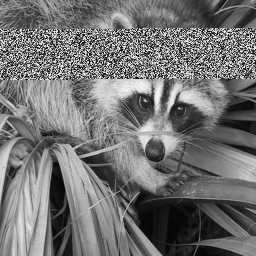
\includegraphics[width=0.3\textwidth]{face_2.png}}
    \end{subcaptionbox}
    \hfill
    \begin{subcaptionbox}{An unrecoverable bitmap image with many small corrupt areas.}
        {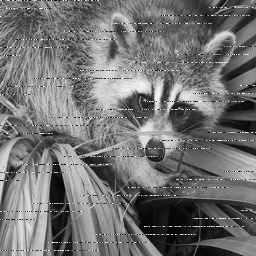
\includegraphics[width=0.3\textwidth]{face_3.png}}
    \end{subcaptionbox}
    \hfill
    \begin{subcaptionbox}{Figure (a), repaired.}
        {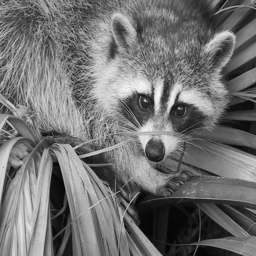
\includegraphics[width=0.3\textwidth]{face_2_repaired.png}}
    \end{subcaptionbox}
    
    \caption{Image source: \texttt{scipy.datasets.face} (derived from \url{https://pixnio.com/fauna-animals/raccoons/raccoon-procyon-lotor})}
\end{figure}

\clearpage

\section{Dependencies}

\label{appendix:dependencies}

The following Rust libraries were used in the implementation:

\begin{itemize}
    \item \texttt{fastrand} - Random number generation for testing.
    \item \texttt{blake3} - Hashing for error detection.
    \item \texttt{crossbeam-channel} - Channels for communication between threads. Although the standard library provides channels, multi-producer multi-consumer channels are not stabilized yet (as of Rust 1.87.0).
    \item \texttt{indicatif} - Terminal progress bars.
    \item \texttt{memmap2} - Cross-platform memory mapped I/O.
    \item \texttt{num\_cpus} - Obtains of CPU cores for automatically selecting number of threads.
    \item \texttt{positioned-io} - Cross-platform random access file I/O.
    \item \texttt{sysinfo} - Obtains available memory for automatically selecting number of codes to process at once.
\end{itemize}

\section{Unit Tests}

\label{appendix:unit}

The following unit tests are used to validate the finite field and polynomial transform algorithms, using Rust's built-in unit testing framework:

\begin{itemize}
\item Addition is commutative.
\item Inverting 0 raises an error.
\item $1^{-1} = 1$.
\item Euclidean algorithm inversion agrees with $x^{2^{64} - 2}$ inversion.
\item $x * x^{-1} = 1$.
\item $(x_1 * x_2 * \ldots * x_n) * (x_1^{-1} * x_2^{-1} * \ldots * x_n^{-1}) = 1$, with the multiplications performed in a random order.
\item Multiplication is commutative.
\item Oversampling a polynomial using the inverse and forward transforms agrees with standard polynomial evaluation.
\item The formal derivative obtained by applying the inverse transform, performing the derivative in the non-monomial basis, then applying the forward transform, agrees with the standard formal derivative.
\item Data recovery using the encoding and decoding algorithms correctly recovers the lost data (test performed in-memory, with no I/O), with various numbers of errors, including the maximum possible number of errors.
\item Attempting to recover lost data with just one error over the maximum error limit results in incorrect data.
      Data recovery fails with too many errors because it attempts to interpolate a polynomial of degree greater than or equal with $n$ with only $n$ values, when at least $n + 1$ values would be needed.
\item When interpolating an oversampled polynomial, the excess coefficients are all zero.
\item Roundtrip test of the forward and inverse transforms - when each is applied the same amount of times, in a random order, the output is the same as the input.
\end{itemize}
